%\documentclass[11pt]{exam}
\documentclass[11pt,answers]{exam}
%Add the ``answers'' flag as above to render your solutions (everything in a
%solution environment)
%Otherwise, only the questions will be rendered

% This header contains many macros useful in Math and Computer Science.
% They may be useful for you to use, and to help learn LaTeX. 
% You don't have to learn them all, but I may use them in the questions below.

\input{hwheader}


% Below are some additional, homework-specific Macros.

\begin{document}
%Your information goes here
\hwheader{Homework 2}{CISC 380}{Dr. Sarah Miracle}{Lennart Buhl}{Jack Lewis}
\noindent {\bf Purpose:} 
 \begin{itemize}
 \item Practice solving recurrence relations.
 \item Learn to design (and analyze) algorithms using a divide and conquer approach.
 \end{itemize}

\hrule
\vspace{2em}

\noindent {\bf General Homework Policies:}
\begin{itemize}
\item This homework assignment is due by the deadline given in Canvas.  Late assignments will not be accepted and will receive a 0.
\item Submit \textbf{two} files through Canvas:
\begin{enumerate}
\item The \texttt{pdf} for the written portion of the assignment (it should generated by modifying the the LaTeX file for this assignment).
\item The completed \texttt{Assignment2.java} file.  Before submitting please zip the java file and submit a \texttt{.zip} file.  See the \emph{Additional Programming Instructions} section below for more detailed instructions.
\end{enumerate}
\item \textcolor{blue}{You will be assigned a partner for this assignment.}  Only one assignment should be submitted and you and your partner will both receive the same grade.   Make sure to include your partner's name on the homework.  Your assignment should be a true joint effort, equally created, and understood by both partners. 
\item You are not allowed to consult outside sources, other than the textbook, your notes, the Java API and the references linked from Canvas (i.e., no looking for answers on the internet).$^1$
\item Getting \emph{ANY} solutions from the web, previous students etc. is \emph{NOT} allowed.$^1$ 
\item Copying code from anywhere or anyone is not allowed (even previous code you have written).  Allowing someone to copy your code is also considered cheating.$^1$
\item You are not allowed to discuss this assignment with anyone except for your partner (if you have one) or the instructor.$^1$
\item Your work will be graded on correctness and clarity.  Write complete and precise answers and show all of your work (there is a detailed grading rubric included at the end of the assignment).  
\item Questions marked (PRACTICE) will not be graded and do not need to be submitted.  However it's highly recommended that you complete them.
\end{itemize}
\emph{$^1$See the section of the syllabus on academic dishonesty for more details.}\\
\hrule
\vspace{2em}
\noindent {\bf Homework Problems:}\\ 
\begin{questions}
\question[3]
  Solve the following recurrences, using the \textbf{recursion tree} method. You should give a $\Theta$ bound.  Show your work and justify your answers (this should include justifying why your answer is a lower AND an upper bound).  Your solution must include a drawing of the recursion tree with at least 3 levels.  \begin{parts}
    \part $T(n) = T(n/5) + T(n/3) + n$ 
    \begin{solution}
      
      
      
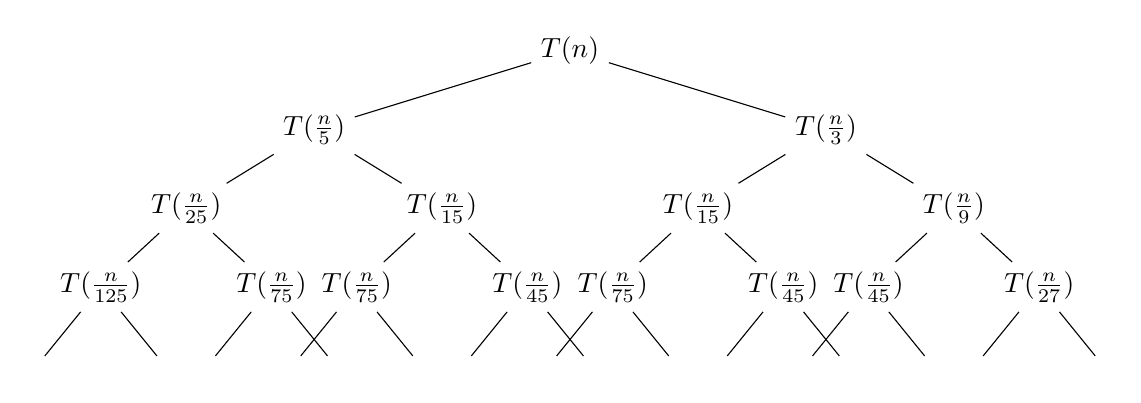
\begin{tikzpicture}[level/.style={sibling distance=65mm/#1, level distance=10mm}]
  \node (z){$T(n)$}
    child {node (a) {$T(\frac{n}{5})$}
      child {node (a1) {$T(\frac{n}{25})$}
        child {node {$T(\frac{n}{125})$}
          child {node {$\hdots$}}  
          child {node {$\hdots$}}  
        }
        child {node {$T(\frac{n}{75})$}
          child {node {$\hdots$}}  
          child {node {$\hdots$}}  
        }
      }
      child {node (a2) {$T(\frac{n}{15})$}
        child {node {$T(\frac{n}{75})$}
          child {node {$\hdots$}}  
          child {node {$\hdots$}}  
        }
        child {node {$T(\frac{n}{45})$}
          child {node {$\hdots$}}  
          child {node {$\hdots$}}  
        }
      }
    }
    child {node (b) {$T(\frac{n}{3})$}
      child {node (b1) {$T(\frac{n}{15})$}
        child {node {$T(\frac{n}{75})$}
          child {node {$\hdots$}}  
          child {node {$\hdots$}}  
        }
        child {node {$T(\frac{n}{45})$}
          child {node {$\hdots$}}  
          child {node {$\hdots$}}  
        }
      }
      child {node (b2) {$T(\frac{n}{9})$}
        child {node {$T(\frac{n}{45})$}
          child {node {$\hdots$}}  
          child {node {$\hdots$}}  
        }
        child {node {$T(\frac{n}{27})$}
          child {node {$\hdots$}}  
          child {node {$\hdots$}}  
        }
      }
    };
\end{tikzpicture}

At each level we have to add $n$ of work, as dictated by the recurrence relation. We can also estimate that the depth of the tree will be $\log_5(n)$, based on the dominating recursion call of $T(n/5)$. 

Now, for the time complexity, we must get the product of the depth of the tree and the amount of work per level inside the tree. The amount of work per level inside the tree is going to be: $T(n/5) + T(n/3) \underline{\textbf{+ n}}$. Similarly, the depth of the tree can be defined by the division within the recurrence: $\log_5(n)$. Therefore, by multiplying $n$ with $\log_5(n)$ we get the following time complexity: $O(n\log_5(n))$
      
    \end{solution}
        \part (\emph{PRACTICE}) $T(n) = 23 T(n/4) + \sqrt{n}.$
        
        \begin{solution}


\begin{tikzpicture}[level/.style={sibling distance=45mm/#1, level distance=10mm}]
  \node {$T(n)$}
    child {node {$T(\frac{n}{4})$}
      child {node {$\vdots$}}
    }
    child {node {$T(\frac{n}{4})$}
      child {node {$\vdots$}}
    }
    child {node {$\cdots \textit{more recursive calls} \; \cdots$}
      child {node {$\vdots$}}
    }
    child {node {$T(\frac{n}{4})$}
      child {node {$\vdots$}}
    };
\end{tikzpicture}

The $T(n) = 23 T(n/4)$ implies that we have 23 recursive calls per level. Another way to write it is as follows: $T(n) = T(n/4) + T(n/4) + T(n/4) + ... + T(n/4) +  \sqrt{n}.$ Another thing we have to keep in mind is that at each level we add $\sqrt{n}$ amount of work, based on the recurrence relation. 

Now, we will apply the master theorem $T(n) \in \Theta(n^{\log_{b}(a)})\; if \; a > b^k$. Since 23(a) $> 4^{0.5}$ we will get the following time complexity: $O(n^{\log_{4}{23}})$.
        \end{solution}
        \part (\emph{PRACTICE}) $T(n) = T(n-1) + 3^n.$
        \begin{solution}

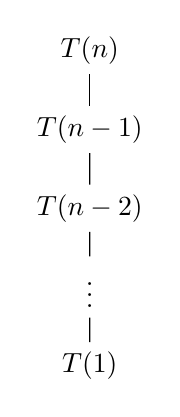
\begin{tikzpicture}[level distance=10mm]
  \node {$T(n)$}
    child {node {$T(n-1)$}
      child {node {$T(n-2)$}
        child {node {$\vdots$}
          child {node {$T(1)$}}
        }
      }
    };
\end{tikzpicture}

Keep in mind that at each level we would add $3^n$ of work. 

Since we are calling things recursively and are not dividing the $n$ by anything, but rather are just subtracting $1$ per level, we can derive the time complexity by getting the product of the amount of work per level and the depth of the recursion tree. Therefore, the time complexity should be $O(3^n)$.
        \end{solution}
        \footnote{For practice problem 2: The reason time complexity is not $O(n*3^n)$ is because that would imply at each level we have work of $3^n$, but at each level we have (n-1) work compared to the previous level. So, we are reducing the amount of work needed the deeper the levels go. Therefore, we choose the highest value (most dominant) of the $3^n+3^{n-1}+3^{n-2}+...+3^1$, which is $3^n$.}
          \end{parts}

  
		\question[7] An array $A[1 \ldots n]$ is said to have a \emph{dominating entry}
  if more than half of its entries are the same.  Given an array, the task is
  to design an efficient algorithm to tell whether the array has a dominating
  entry, and, if so, to find that entry or element.  The elements of the array
  are abstract objects, and not necessarily from some ordered domain like the
  integers, and so there can be no comparisons of the form ``is $A[i] >
  A[j]$?" (this means that you cannot any sorting algorithms like Bubble Sort, Merge Sort etc.). However you can answer questions of the form: ``is A[i] = A[j]?" in
  constant time.  Show how to solve this problem in $O(n\log n)$ time using a \textbf{divide and conquer} approach.  
     \begin{parts}
    \part Explain your algorithm in words and justify why it is correct. 
    \begin{solution}
      
      Suppose we have a bag of marbles. We want to check if we have a dominant color. We can either count all of the marbles and keep track of the colors and their corresponding occurrence, or we can use a divide and conquer algorithm to help us. We first split the bag in half. If we have only a few marbles we can quickly identify a dominant color in each bag. If we still have a lot of marbles, we can continue to split or \textbf{divide} the bags until they are small enough for us to count easily. Now, we find the dominant color of the small bags. If we compare the two leaf bags (who have the same parent bag) and both of them have \textit{blue} as the dominant color, then \textit{blue} is the dominant color of the parent bag. We are now essentially moving back up the latter and comparing the bags based on their leaf bags. If one bag is \textit{blue} and the other is \textit{green} then we must count all of the marbles to assess a winner. If there is no winner then there is no single dominant color in that particular bag.  \\
      
      So, how does this apply to our algorithm? Well, we also use a divide and conquer algorithm where we first divide the problem into smaller and smaller sub-problems. We then \textit{conquer} each sub-problem by recursively finding a potential dominating entry. And then finally, we combine the results by counting the occurrences of these entries to confirm if one is truly dominating. This approach will result in $O(n\log(n))$ time because the depth of the algorithm is defined by the amount of divides and the amount of work per level. Since the work per level is $n$ and the depth of the algorithm will be $\log_2(n)$ we can savely assume that the result is $O(n\log_2(n))$ time.
      
      
    \end{solution}
		\part Provide well-commented pseudocode.
		 \begin{solution}
     \vspace{-0.2cm}
     \begin{verbatim}
function findDominantElement(array, start, end)
  # basecase - if array only has one element,
  # then the element is dominant entry
  if start == end
    return array[start]
  
  # find simple midpoint
  mid = (start + end) / 2
  # recursiveyl find the left/right hand dominant element
  leftDominant = findDominantElement(array, start, mid)
  rightDominant = findDominantElement(array, mid+1, end)
  
  # if both halves have the same dominant element,
  # then we know that's the dominant element of the whole.
  # So, we simply return the dominant element.
  if leftDominant == rightDominant
    return leftDominant

  # count the occurences of the dominant elements in the array
  leftCount = countOccurrences(array, start, end, leftDominant)
  rightCount = countOccurrences(array, start, end, rightDominant)
  
  # if the left/right dominant element appears more than
  # half in the array,
  # we have found the dominant element of the array
  # So, we return the dominant element
  half = (end - start + 1) / 2
  if leftCount > half
    return leftDominant
  if rightCount > half
    return rightDominant
  
  # If we do not find a dominant element we return null
  return null
\end{verbatim}

    \end{solution}
    \part Analyze your algorithm including stating and solving the relevant recurrence relation (and justifying your analysis).    
		\begin{solution}


Since the divide step is $O(1)$ time and we have two recursive calls, which halve the array we can say the following: $T(n) = 2T(n/2) + n$. We have the $+ n$ because of the counting we are doing which happens in linear time. From \textit{start} to \textit{finish} $\rightarrow O(n)$ . \\

Now, based on our division by the two recursive call, we can know that the depth of the tree will only go up to $log_2(n)$ and we have a linear counting algorithm which is $O(n)$. Since we are finding the product between the depth and the amount of work per level, we can come to the following solution:\\
$O(\log(n)) \times O(n) = O(n*\log(n))$\\
\textit{Or, to be more precise:}\\    
$O(\log_2(n)) \times O(n) = O(n*\log_2(n))$\\
    
    \end{solution}
    \footnote{Assuming that we are generally referring to $log_{10}$ when speaking about $log$.}
    \part (\emph{EXTRA CREDIT}) Implement your pseudo-code from part (b).  Add code to the \texttt{dominant} method in the \texttt{Assignment2.java} file provided with the assignment.  Note that for simplicity you are implementing this algorithm for an array of integers.  However, you are still not allowed to compare elements in the array only to check for equality (i.e. no $A[i] > A[j]$).
  \end{parts}
     \question[5]  Recall the maximum subarray problem discussed in class (given (possibly negative) integers $a_1, a_2, \ldots, a_n$, find the maximum value of $\sum_{k=i}^j a_k$).  You will design and implement a \textbf{divide and conquer} algorithm to solve this problem.  Your algorithm should divide the array in half as in Merge Sort and have running time $\Theta(n\log n).$  Complete the partial code given to you in the \texttt{maxSubArrayRecursive} method within file \texttt{Assignment2.java}.  Note that if the array contains only negative numbers then the answer should be negative.  For example, if the input is \texttt{[-1, -2, -3]} then your method should return -1 (i.e. a subarray has length at least 1).

\question[6] You're given an array of $n$ numbers. A $hill$ in this array is an element
    $A[i]$ that is at least as large as it's neighbors. In other words,
    $A[i] \geq A[i-1]$ and $A[i] \geq A[i+1]$.
    (If $i=1$ is a hill then we only need $A[1] \geq A[2]$, resp. if $i = n$
    is a hill if $A[n] \geq A[n-1]$.)  Consider the following divide \& conquer algorithm that solves the hill problem:
    
\emph{If $n \leq 2$, then return the larger (or only) element in the array. 
        Otherwise compare the two elements in the middle of the array,
        $A[\frac{n}{2} -1]$ and $A[\frac{n}{2}]$. If the first is bigger, then
        recurse in the first half of the array, otherwise recurse in the
        second half of the array.}
        
Why is this a valid solution?  Think about why this algorithm is correct. \\

For this problem, you will implement two different solutions for the hill problem.  You will add code to the \texttt{Assignment2.java} file provided with the assignment.  
    \begin{parts}
      \part Give a \textbf{brute force} algorithm that can find a hill. As a comment at the top of the \texttt{bruteHill} method explain your algorithm in words and analyze its running time.  Then implement your algorithm by adding code to the \texttt{bruteHill} method.
      \part Implement the divide and conquer algorithm given in Problem~4 by adding code to the 
      \texttt{divideAndConquerHill} method.  Note that you will need to modify the algorithm given above slightly to return the index of the hill instead of the element.  As a comment at the top of the \texttt{divideAndConquerHill} method state the recurrence relation and analyze its running time. 
      \end{parts}
      Code is given in the \texttt{Assignment2HillDriver.java} file that compares the performance of the two methods.  You should run this code and think about the output.  Note that the code does not thoroughly test your methods - this is something you should do!   \\
      
       \end{questions}

\noindent {\bf Additional Programming Instructions:}\\ 

\noindent Note that your code will be automatically run on a standard set of test cases.  In order to ensure that you do not lose points, follow the instructions below.
\begin{itemize}
\item Your code must compile without any errors using the version of Java on the lab computers.  If your code does not compile you will not receive any points for the assignment.
\item Do not modify any of the methods signatures (i.e. name, return type or input type).  Note that you are always welcome (and encouraged) to add additional methods but these will not be run directly by the test code.
\item You are not allowed to use packages (e.g. no statement \texttt{package ...} at the top of your file).
\item No extra folders or files in your submission.  Zip up only the files you need to submit not the folder they are in.
\item Your solution should not print anything unless explicitly instructed to.
\end{itemize}
      \hrule
\vspace{2em}
\noindent {\bf Grading Criteria:}\\

\vspace{.5em}

\noindent Your work will be graded on both correctness {\bf and clarity}.  Write complete and precise answers and show all of your work.  Your pseudo-code and proofs should follow the guidelines posted on Canvas and discussed in class.    \\

Evaluation Rubric for Problem 1\\
\begin{center}
  \begin{tabular}{| p{7cm} | p{10cm} |}
	\hline
	Component & Requirement for Full Credit\\
    \hline
    Solution Correctness  (1pt) & The answer is correct. \\ \hline
  Written Explanation  (2pt) & Your solution includes a logical argument explaining why your answer is correct. The explanation is clear, correct and complete.   It includes full sentences and is easily understood by any student in the class. Think of this as a proof and remember what you learned in Math 128. Note that you must include a drawing of the recursion tree with at least 3 levels.  Additionally you must justify why your answer is a tight-bound (i.e., just arguing that the run time is big-O is not enough)\\ \hline
  \end{tabular}
\end{center} 

Evaluation Rubric for Problem 2\\
\begin{center}
  \begin{tabular}{| p{7cm} | p{10cm} |}
	\hline
	Component & Requirement for Full Credit\\
    \hline
    Solution Correctness  (3pts) & The algorithm will work correctly on all inputs and uses a divide and conquer strategy.  \\ \hline
  Written Description \& Justification (2pt) & The explanation of the algorithm and why it is correct is clearly written and easily understandable.  It includes full sentences and should be easily understood by any student in the class. \\ \hline
	Pseudo-code  (1pt) & The pseudo-code is clearly written following the guidelines discussed in class.\\ \hline
	Running Time Analysis  (1pt) & The solution gives a recurrence relation and solves it.  It is clearly written and correct (for the algorithm given!).  \\ \hline
	Implementation (EXTRA CREDIT)  (1pt) & Your code will be run on a standard set of test cases.  Make sure to test your code thoroughly!  Note that you will lose points if you do not follow the general style guidelines given in the syllabus or if your implementation changes the running time of your pseudo-code.  You will receive NO credit if your code does not implement your pseudo-code (which must use a divide and conquer approach) or if you compare elements in the array directly.  \\ \hline

  \end{tabular}
\end{center}

Evaluation Rubric for Problem 3.
\begin{center}
  \begin{tabular}{| p{7cm} | p{10cm} |}
	\hline
	Component & Description 	\\
    \hline
    Style \& Documentation  (1 pts) & I'll be watching for style issues as well as correct output.  See the syllabus for some general style guidelines (e.g. your code should be well-documented).  
		\\ \hline
 Correct Output on Test Cases* (4 pt) & Your code will be run on a standard set of test cases. \\ \hline
  \end{tabular}
\end{center}
*Note that if your code does not implement a divide and conquer algorithm (using the given starter code) with the appropriate running time, you will lose credit regardless of whether the test cases execute correctly.\\

Evaluation Rubric for Problem 4.
\begin{center}
  \begin{tabular}{| p{7cm} | p{10cm} |}
	\hline
	Component & Description 	\\
    \hline
    Style \& Documentation  (1 pts) & I'll be watching for style issues as well as correct output.  See the syllabus for some general style guidelines (e.g. your code should be well-documented).  \\ \hline
	\textcolor{black}{\emph{brute force} Description \& Big-O Analysis (1 pt)} & \textcolor{black}{Your \emph{brute force} algorithm explanation should be in full sentences and contain as much detail as pseudo-code.  Make sure to justify your analysis as well as given a bound (i.e., explain where your bound comes from and why it is correct).}\\ \hline
	\textcolor{black}{\emph{divide \& conquer} Big-O Analysis (1 pt)} & \textcolor{black}{Make sure to justify your analysis as well as given a bound.  This must include stating (and justifying) a recurrence relation as well as solving it.  If applicable, you may use the Master Theorem but make sure to state which case you are using and show your work.  Note that your run time should be the best asymptotic time possible given the pseudo-code.  Otherwise, you will lose points even if your analysis is correct.}\\ \hline
 Correct Output on Test Cases* (2 pt) & Your \emph{brute force} code will be run on a standard set of test cases. \\ \hline
	Correct Output on Test Cases* (2 pt) & Your \emph{divide \& conquer} code will be run on a standard set of test cases.\\ \hline
  \end{tabular}
\end{center}
*Note that if your code does not implement the appropriate algorithm you will receive no credit regardless of whether the test cases execute correctly.

\end{document}
